

\tikzset{every picture/.style={line width=0.75pt}} %set default line width to 0.75pt        

\begin{tikzpicture}[x=0.58pt,y=0.58pt,yscale=-1,xscale=1]
%uncomment if require: \path (0,489); %set diagram left start at 0, and has height of 489

%Shape: Ellipse [id:dp9714732770479797] 
\draw   (22,140.42) .. controls (22,121.87) and (66.77,106.83) .. (122,106.83) .. controls (177.23,106.83) and (222,121.87) .. (222,140.42) .. controls (222,158.97) and (177.23,174.01) .. (122,174.01) .. controls (66.77,174.01) and (22,158.97) .. (22,140.42) -- cycle ;
%Straight Lines [id:da9470856219208896] 
\draw    (284,60) -- (176.77,104.84) ;
\draw [shift={(174,106)}, rotate = 337.31] [fill={rgb, 255:red, 0; green, 0; blue, 0 }  ][line width=0.08]  [draw opacity=0] (10.72,-5.15) -- (0,0) -- (10.72,5.15) -- (7.12,0) -- cycle    ;
%Shape: Ellipse [id:dp39391125687327155] 
\draw   (163,214.91) .. controls (163,194.43) and (207.77,177.83) .. (263,177.83) .. controls (318.23,177.83) and (363,194.43) .. (363,214.91) .. controls (363,235.4) and (318.23,252) .. (263,252) .. controls (207.77,252) and (163,235.4) .. (163,214.91) -- cycle ;
%Straight Lines [id:da6338019201234634] 
\draw    (401,141) -- (325.71,176.71) ;
\draw [shift={(323,178)}, rotate = 334.62] [fill={rgb, 255:red, 0; green, 0; blue, 0 }  ][line width=0.08]  [draw opacity=0] (10.72,-5.15) -- (0,0) -- (10.72,5.15) -- (7.12,0) -- cycle    ;
%Shape: Ellipse [id:dp13655633022849756] 
\draw   (262,215.54) .. controls (262,205.66) and (277.78,197.66) .. (297.25,197.66) .. controls (316.72,197.66) and (332.5,205.66) .. (332.5,215.54) .. controls (332.5,225.42) and (316.72,233.42) .. (297.25,233.42) .. controls (277.78,233.42) and (262,225.42) .. (262,215.54) -- cycle ;
%Shape: Ellipse [id:dp5449944288813106] 
\draw   (183,215.54) .. controls (183,205.66) and (198.78,197.66) .. (218.25,197.66) .. controls (237.72,197.66) and (253.5,205.66) .. (253.5,215.54) .. controls (253.5,225.42) and (237.72,233.42) .. (218.25,233.42) .. controls (198.78,233.42) and (183,225.42) .. (183,215.54) -- cycle ;
%Straight Lines [id:da030702262544070935] 
\draw    (317,61) -- (408.27,102.75) ;
\draw [shift={(411,104)}, rotate = 204.58] [fill={rgb, 255:red, 0; green, 0; blue, 0 }  ][line width=0.08]  [draw opacity=0] (10.72,-5.15) -- (0,0) -- (10.72,5.15) -- (7.12,0) -- cycle    ;
%Straight Lines [id:da1564630306712015] 
\draw    (434,142) -- (518.27,180.75) ;
\draw [shift={(521,182)}, rotate = 204.69] [fill={rgb, 255:red, 0; green, 0; blue, 0 }  ][line width=0.08]  [draw opacity=0] (10.72,-5.15) -- (0,0) -- (10.72,5.15) -- (7.12,0) -- cycle    ;
%Shape: Ellipse [id:dp6368613727912615] 
\draw   (289,308.91) .. controls (289,290.09) and (327.28,274.83) .. (374.5,274.83) .. controls (421.72,274.83) and (460,290.09) .. (460,308.91) .. controls (460,327.74) and (421.72,343) .. (374.5,343) .. controls (327.28,343) and (289,327.74) .. (289,308.91) -- cycle ;
%Shape: Ellipse [id:dp08483334028737277] 
\draw   (305,312.54) .. controls (305,302.66) and (320.78,294.66) .. (340.25,294.66) .. controls (359.72,294.66) and (375.5,302.66) .. (375.5,312.54) .. controls (375.5,322.42) and (359.72,330.42) .. (340.25,330.42) .. controls (320.78,330.42) and (305,322.42) .. (305,312.54) -- cycle ;
%Shape: Ellipse [id:dp4660930800548526] 
\draw   (389,309) .. controls (389,290.22) and (420.79,275) .. (460,275) .. controls (499.21,275) and (531,290.22) .. (531,309) .. controls (531,327.78) and (499.21,343) .. (460,343) .. controls (420.79,343) and (389,327.78) .. (389,309) -- cycle ;
%Straight Lines [id:da5096569303441225] 
\draw    (515,220) -- (423.68,265.66) ;
\draw [shift={(421,267)}, rotate = 333.43] [fill={rgb, 255:red, 0; green, 0; blue, 0 }  ][line width=0.08]  [draw opacity=0] (10.72,-5.15) -- (0,0) -- (10.72,5.15) -- (7.12,0) -- cycle    ;
%Shape: Ellipse [id:dp5549354135393528] 
\draw   (594,307.91) .. controls (594,289.09) and (630.71,273.83) .. (676,273.83) .. controls (721.29,273.83) and (758,289.09) .. (758,307.91) .. controls (758,326.74) and (721.29,342) .. (676,342) .. controls (630.71,342) and (594,326.74) .. (594,307.91) -- cycle ;
%Shape: Ellipse [id:dp22039734942458056] 
\draw   (608,311.54) .. controls (608,301.66) and (623.78,293.66) .. (643.25,293.66) .. controls (662.72,293.66) and (678.5,301.66) .. (678.5,311.54) .. controls (678.5,321.42) and (662.72,329.42) .. (643.25,329.42) .. controls (623.78,329.42) and (608,321.42) .. (608,311.54) -- cycle ;
%Shape: Ellipse [id:dp5560061601595019] 
\draw   (687,308) .. controls (687,289.22) and (714.31,274) .. (748,274) .. controls (781.69,274) and (809,289.22) .. (809,308) .. controls (809,326.78) and (781.69,342) .. (748,342) .. controls (714.31,342) and (687,326.78) .. (687,308) -- cycle ;
%Straight Lines [id:da6023491908932058] 
\draw    (572,219) -- (674.24,262.82) ;
\draw [shift={(677,264)}, rotate = 203.2] [fill={rgb, 255:red, 0; green, 0; blue, 0 }  ][line width=0.08]  [draw opacity=0] (10.72,-5.15) -- (0,0) -- (10.72,5.15) -- (7.12,0) -- cycle    ;
%Shape: Ellipse [id:dp055919448535677874] 
\draw   (701,309.33) .. controls (701,297.91) and (710.63,288.66) .. (722.5,288.66) .. controls (734.37,288.66) and (744,297.91) .. (744,309.33) .. controls (744,320.74) and (734.37,330) .. (722.5,330) .. controls (710.63,330) and (701,320.74) .. (701,309.33) -- cycle ;

% Text Node
\draw    (265,22.5) -- (329,22.5) -- (329,60.5) -- (265,60.5) -- cycle  ;
\draw (268,26.5) node [anchor=north west][inner sep=0.75pt]   [align=left] {P $\displaystyle \overset{?}{=}$NP};
% Text Node
\draw (36,133.5) node [anchor=north west][inner sep=0.75pt]   [align=left] {P $\displaystyle =$NP$\displaystyle =$co-NP$\displaystyle =$NPC};
% Text Node
\draw    (368,103.5) -- (464,103.5) -- (464,141.5) -- (368,141.5) -- cycle  ;
\draw (371,107.5) node [anchor=north west][inner sep=0.75pt]   [align=left] {NP $\displaystyle \overset{?}{=}$co-NP};
% Text Node
\draw (218,250.5) node [anchor=north west][inner sep=0.75pt]   [align=left] {NP$\displaystyle =$co-NP};
% Text Node
\draw (292.12,208.56) node [anchor=north west][inner sep=0.75pt]   [align=left] {P};
% Text Node
\draw (202.12,207.56) node [anchor=north west][inner sep=0.75pt]   [align=left] {NPC};
% Text Node
\draw    (478,181.5) -- (602,181.5) -- (602,219.5) -- (478,219.5) -- cycle  ;
\draw (481,185.5) node [anchor=north west][inner sep=0.75pt]   [align=left] {P $\displaystyle \overset{?}{=}$NP$\displaystyle \cap $co-NP};
% Text Node
\draw (363,344.5) node [anchor=north west][inner sep=0.75pt]   [align=left] {NP};
% Text Node
\draw (420.12,303.56) node [anchor=north west][inner sep=0.75pt]   [align=left] {P};
% Text Node
\draw (324.12,304.56) node [anchor=north west][inner sep=0.75pt]   [align=left] {NPC};
% Text Node
\draw (444,345.5) node [anchor=north west][inner sep=0.75pt]   [align=left] {co-NP};
% Text Node
\draw (665,343.5) node [anchor=north west][inner sep=0.75pt]   [align=left] {NP};
% Text Node
\draw (718.12,302.56) node [anchor=north west][inner sep=0.75pt]   [align=left] {P};
% Text Node
\draw (627.12,303.56) node [anchor=north west][inner sep=0.75pt]   [align=left] {NPC};
% Text Node
\draw (730,343.5) node [anchor=north west][inner sep=0.75pt]   [align=left] {co-NP};
% Text Node
\draw (211,65) node [anchor=north west][inner sep=0.75pt]   [align=left] {Y};
% Text Node
\draw (363,64) node [anchor=north west][inner sep=0.75pt]   [align=left] {N};
% Text Node
\draw (346,146) node [anchor=north west][inner sep=0.75pt]   [align=left] {Y};
% Text Node
\draw (446,231) node [anchor=north west][inner sep=0.75pt]   [align=left] {Y};
% Text Node
\draw (482,145) node [anchor=north west][inner sep=0.75pt]   [align=left] {N};
% Text Node
\draw (629,225) node [anchor=north west][inner sep=0.75pt]   [align=left] {N};


\end{tikzpicture}

